\section{Wealth Shares}\label{secIA:WealthShares}

There are two state variables in our demand disagreement model: (i) the exogenous fraction of newborn patient investors $\alpha_t$ and (ii) the endogenous consumption share of patient investors $f_t$. Instead of the consumption share we could have also used the wealth share of patient investors as the endogenous state variable. Specifically, the wealth share of patient and impatient investors is
\begin{align*}
	f^W_t &= \frac{1}{W_t} \int_{-\infty}^t \nu  e^{-\nu(t-s)}    \alpha_s W_{s,t}^a \: ds =   \frac{f_t}{\beta^a_t} = \frac{1}{1 + \frac{\nu+\rho_a}{\nu+\rho_b} \frac{1-f_t}{f_t}}. 
\end{align*}
and
\begin{align*}
	1-f^W_t  = \frac{1}{W_t} \int_{-\infty}^t \nu  e^{-\nu(t-s)}   (1-\alpha_s) W_{s,t}^b \: ds   =  \frac{1-f_t}{\beta^b_t}
	= \frac{1}{1 + \frac{\nu+\rho_b}{\nu+\rho_a} \frac{f_t}{1-f_t}},
\end{align*}
respectively. The left graph of Figure \ref{fig:WealthShare} shows the wealth share of patient investors and the right graph shows the consumption share for comparison.  
\begin{figure}[htbp]
\centering
\vspace{0.1in}
\begin{tabular}{cc}
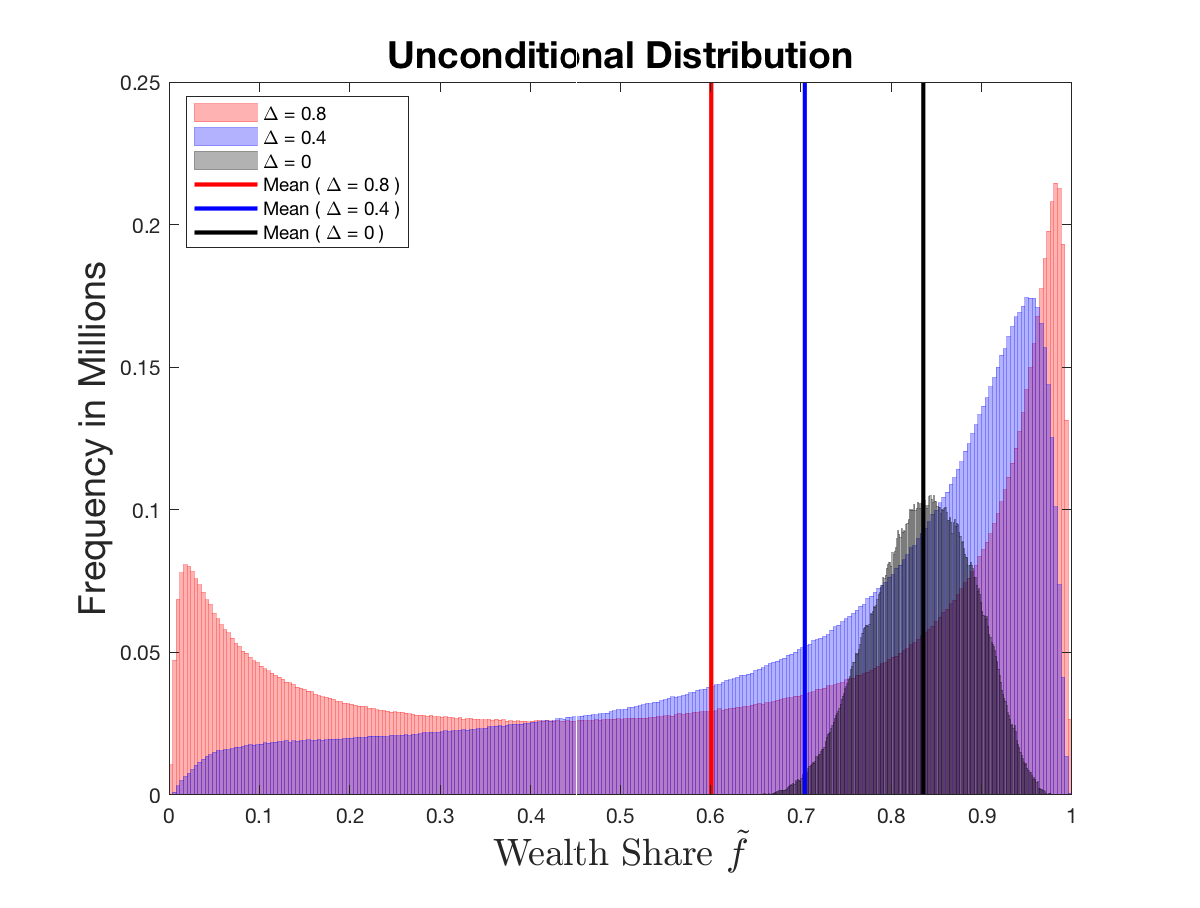
\includegraphics[width=.4\textwidth]{figures/ftWhist.eps} &
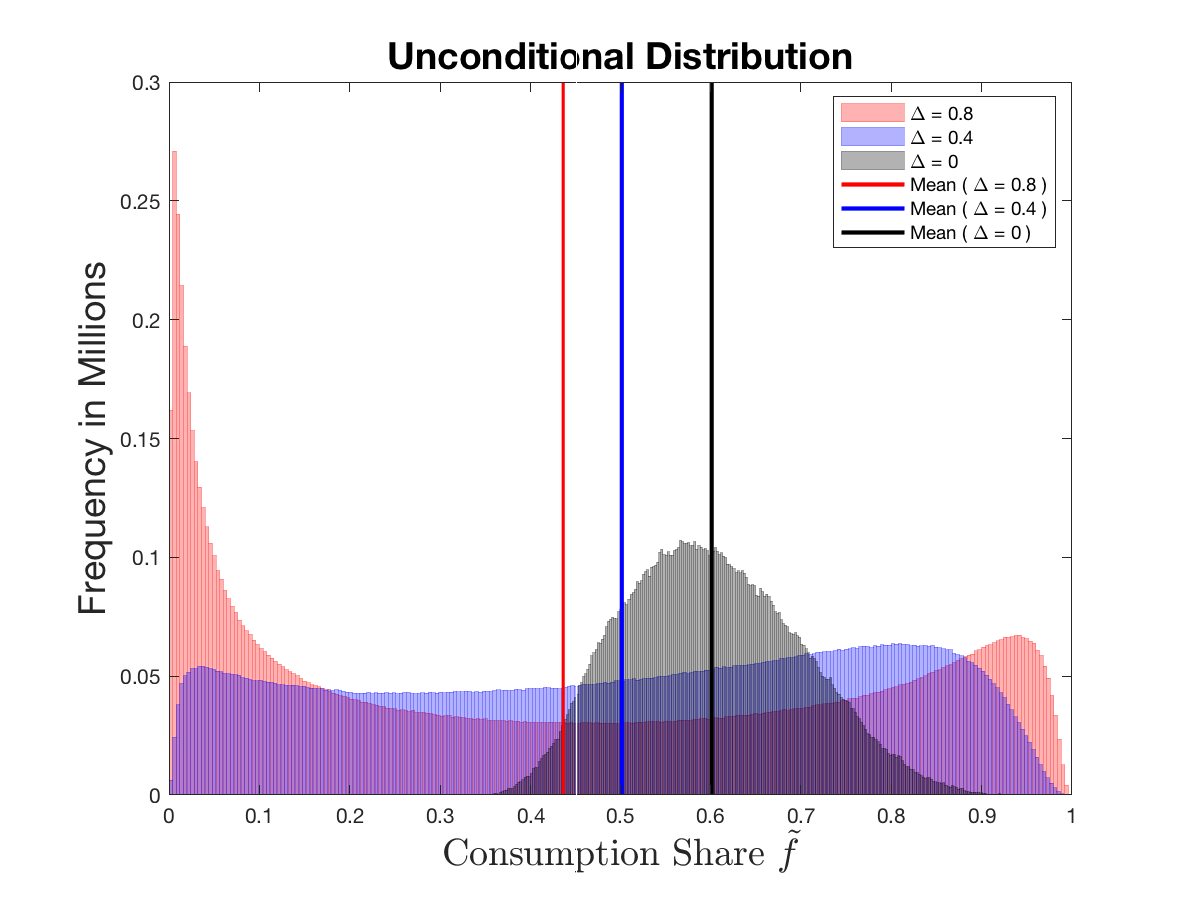
\includegraphics[width=.4\textwidth]{figures/ftHist.eps} \\
\end{tabular}
\caption{\textbf{The Wealth/Consumption share.} \footnotesize{The left graph shows the unconditional distribution of the wealth share $\tilde{f}^W$ and the right graph shows the unconditional distribution of the consumption share of patient investors $\tilde{f}$. The histograms are based one million years of monthly observations for each value of disagreement $\Delta$.  In this example the parameters are based on the alternative calibration with $\rho^a = 0.001$ and $\rho^b = 0.05$}} \label{fig:WealthShare} 
\end{figure}




